\scanpage{67}
\[
-1-(-1)\;/\;0\;/\;1\mathrel{\vert\!\!-}0
\qquad -\frac{1}{4i}(i-1)^2=\frac12
\]
\diagram{\begin{tikzcd}[ampersand replacement=\&, column sep=large]
X_2\arrow[r,no head,"z\mapsto z^2"]\&X_1\arrow[r]\&X_0
\end{tikzcd}}
\[
\begin{array}{ccc}
0&0\mid\infty&\infty\\
1\quad-1&1&0\\
\infty&\deleted{\unsure{-1|\infty}}&1
\end{array}
\qquad\unsure{\text{en}|i}\quad -1+1-2i
\]
\figure{\begin{tikzpicture}[scale=.76, every node/.style={font=\small}]
\begin{scope}[rotate=180,transform shape]
\node[anchor=west]at(0,0){Cartes};\node[anchor=west]at(0,-.7){Cartes orientées};
\node[anchor=west]at(3.3,0){$\unsure{\mathcal G_2|\Gamma_2}$-ens};\node[anchor=west]at(3.3,-.7){$\unsure{\mathcal G_2^0|\Gamma_2^0}$-ens};
\node[anchor=west]at(6.8,0){$\sigma_0^2=\sigma_1^2=\sigma_\infty^2=(\sigma_0\sigma_\infty)^2=1$};
\node[anchor=west,align=left]at(6.8,-.9){$\bigl(\unsure{\rho_0,\rho_1,\rho_\infty|f_0,f_1,f_\infty},$\\$\qquad\unsure{\rho_0\rho_1\rho_\infty=\rho_1^2|f_0f_1f_\infty=f_1^2}=1\bigr)$};
\node[anchor=west]at(3.4,-2.05){$\varphi(z)=\dfrac{z-1}{z+1}$};
\node[anchor=west]at(-.1,-2.1){$\begin{array}{ccc}0&\longrightarrow&1\\1&\mathrel{-}&1\end{array}$};
\node[anchor=west]at(-.15,-3.15){$i,$};
\node[anchor=west]at(.2,-4.05){$\begin{array}{ccc}1&\mathrel{-}&1\\-1&\mathrel{-}&0\\0&\mathrel{-}&\infty\end{array}$};
\node at(2.3,-3.18){$\deleted{\unsure{z}}$};\node at(3.35,-3.8){$\deleted{\unsure{i}}$};
\node[anchor=west]at(3,-4.18){$i,-i\longmapsto\tfrac12$};\node at(3.6,-4.9){$z$};
\node[anchor=west]at(4.7,-5.45){$(0,\infty)$};\node at(5.45,-6.15){$1$};\node at(5.45,-6.8){$0$};
\node at(8,-5.15){$\left(\dfrac{z-1}{z+1}\right)^2$};
\begin{scope}[shift={(8.1,-3.35)}]
\draw(-1.25,0)arc(180:0:1.25 and .95);\draw(-1.25,-.15)arc(180:360:1.25 and .95);\draw(-1.35,-.05)--(1.3,-.05);
\fill(0,-.05)circle(.035);\node[below]at(0,-.06){$0$};\node[left]at(-1.35,-.1){$\unsure{\beta|3}$};\draw(1.3,-.1)--(1.45,-.1);
\end{scope}
\begin{scope}[shift={(-3,-1.9)}]
\draw(-.7,-.5)--(-.75,.4)--(0,.65)--(.7,.38)--(.35,-.5)--cycle;
\draw(-.7,-.5)--(0,.65)--(.35,-.5);\draw(-.7,-.22)--(-.45,.02)--(-.67,.06)--(-.41,.21);\draw(.24,.55)--(.42,.32)--(.47,.49)--(.58,.3)--(.6,.45);
\draw(0,.7)--(.2,1.55);\node at(.25,.97){$0$};\node[below]at(-.7,-.5){$1$};\node[below]at(.35,-.5){$\infty$};
\end{scope}
\begin{scope}[shift={(-3.1,-4.25)}]
\draw(-1,0)arc(180:0:1 and .6);\draw(-1,-.12)arc(180:360:1 and .6);\draw[thick](-1,-.02)--(-.15,-.06);\draw[thick](.15,-.09)--(1.03,-.12);
\fill(-.05,-.07)circle(.025);\node[above]at(-.05,-.08){$0$};\node at(0,.3){$r$};\node at(0,-.4){$\sigma_0r=\sigma_1r$};\node[left]at(-1.06,0){$1$};\node at(-1.2,-.25){$\unsure{\varphi}$};\node[right]at(1.02,-.1){$\infty$};
\end{scope}
\begin{scope}[shift={(-2.4,-7.35)}]
\draw(0,0)circle(1.25);\draw[dashed](-1.17,.3)--(-.1,.2);\fill(-.1,.2)circle(.03);\node[right]at(-.1,.2){$0$};
\draw[thick](-1.15,.25)to[bend right=45](-.25,-.4);
\end{scope}
\draw[very thick](1.35,-6.65)--(3.25,-6.7);\fill(1.35,-6.65)circle(.045);\fill(3.25,-6.7)circle(.045);\node[below]at(1.35,-6.65){$0$};\node[below]at(3.25,-6.7){$1$};
\begin{scope}[shift={(2,-9.4)}]
\draw(0,0)circle(1.48);\draw[dashed](-1.46,.05)arc(180:0:1.46 and .27);\draw(-1.46,.05)arc(180:360:1.46 and .27);
\draw[very thick](-.63,-.18)to[bend right=6](.65,-.19);\fill(-.63,-.18)circle(.075);\fill(.65,-.19)circle(.075);\node[below]at(-.63,-.18){$0$};\node[below]at(.65,-.19){$0$};\node at(0,-.05){$1$};\fill(.07,.3)circle(.035);\node[right]at(.07,.3){$\infty$};
\draw[->](-.05,1.05)--(-.08,1.26)--(-.4,1.06);\node[right]at(.1,1.12){$1\quad-1\quad0.$};
\end{scope}
\begin{scope}[shift={(-1,-12.5)}]
\draw(0,0)ellipse(2 and .8);\draw[very thick](-1.55,-.5)to[bend right=12](.2,-.79);\fill(.2,-.79)circle(.075);\fill(-1.55,-.5)circle(.03);\node[below]at(-1.55,-.5){$1$};\fill(.53,.77)circle(.03);\node[above]at(.53,.77){$\infty$};
\end{scope}
\node at(5.5,-12.75){$\dfrac{\left(\dfrac{z-1}{z+1}\right)^2}{\left(\dfrac{z-1}{z+1}\right)^2-1}$};
\node[align=left]at(8.6,-13.1){$=\dfrac{(z-1)^2}{(z-1)^2-(z+1)^2}$\\[10pt]$=\dfrac{(z-1)^2}{-4z}$};
\draw[thin](-.1,.65)to[bend right=5](-1.7,-9.2)to[bend right=5](-1.9,-14.8);
\draw[thin](7.2,-1.25)to[bend right=6](6.2,-8.8)to[bend right=5](6,-15.4);
\end{scope}
\end{tikzpicture}}
\diagram{\begin{tikzcd}[ampersand replacement=\&, column sep=large]
X_1\arrow[r]\&\mathbb X_1\arrow[r,"z\mapsto z^2"]\&\mathbb X_0\arrow[r,no head,"\psi"]\&\mathbb X_0
\end{tikzcd}}
\[
(0,1,\infty)\longrightarrow(0,1,\infty)\mathrel{\vert\!\!-}\quad0\quad\infty\quad1
\]
\mspage{66}
